

%\pagenumbering{roman} \setcounter{page}{1}
\chapter{Brukerveiledning for headless CMS}
\label{appendix:user-manual}

\section{Introduksjon til systemet}
CMS-et er oppbygget på følgende måte: 

\begin{itemize}
\item CMS-et kan bestå av flere sider (pages).
\item Hver side inneholder en eller flere komponenter (components), som er gjenbrukbare og kan tilhøre flere sider.
\item Hver komponent inneholder felter (fields), som holder på innholdet som vises på siden. Det finnes forskjellig felttyper. For eksempel kan et felt være et bilde, et tekstområde eller en lenke. 
\end{itemize}

Det er bare brukere med rollen superadmin som kan opprette komponenter og felter. Andre roller kan kun velge mellom de ferdigdefinerte komponenter og felter når en ny side skal opprettes.

\section{Legge til ny side}

For å legge til en ny side, trykk på \q{Ny side}-knappen til høyre på siden. 

\begin{figure}[H]
    \centering
    \frame{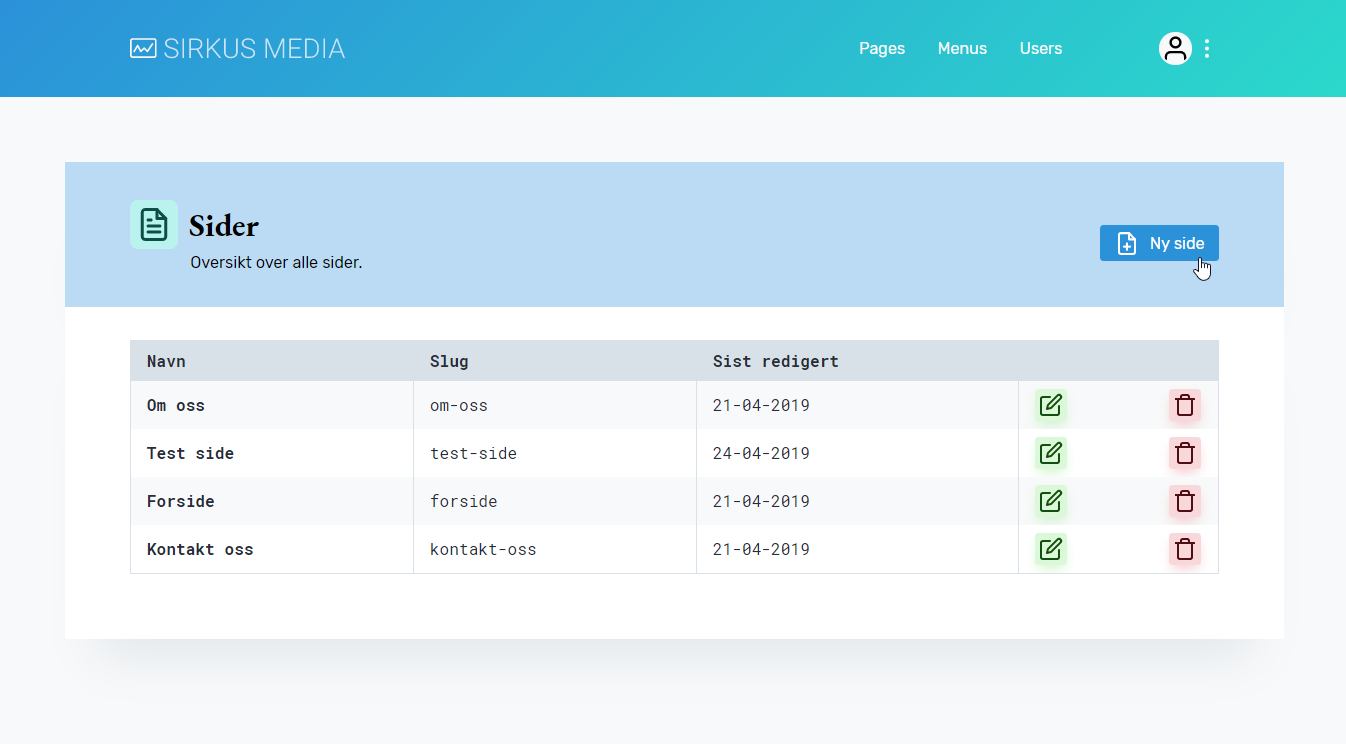
\includegraphics[width=\textwidth]{brukerveiledning/new-page.png}}
    \label{fig:cms-new-page}
\end{figure}

Dette vil føre deg til et nytt vindu. I dette vinduet kan du skrive inn en tittel, som blir den samme tittelen som vises i oversikten. I tillegg kan du legge til den komponenten du ønsker ved å trykke på \q{Legg til komponent}

\begin{figure}[H]
    \centering
    \frame{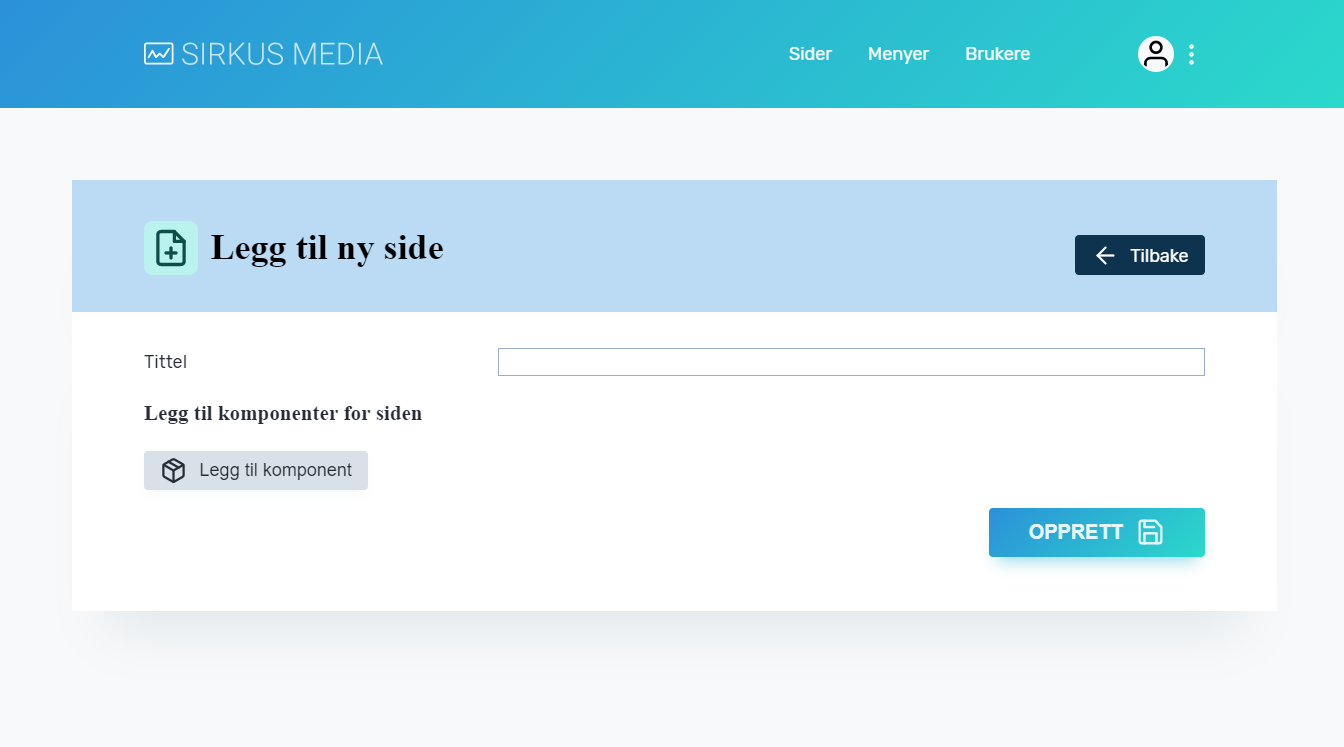
\includegraphics[width=\textwidth]{brukerveiledning/add-component.png}}
    \label{fig:cms-add-component}
\end{figure}

Her må du huke av for den komponenten du ønsker og trykke \q{Velg}.

\begin{figure}[H]
    \centering
    \frame{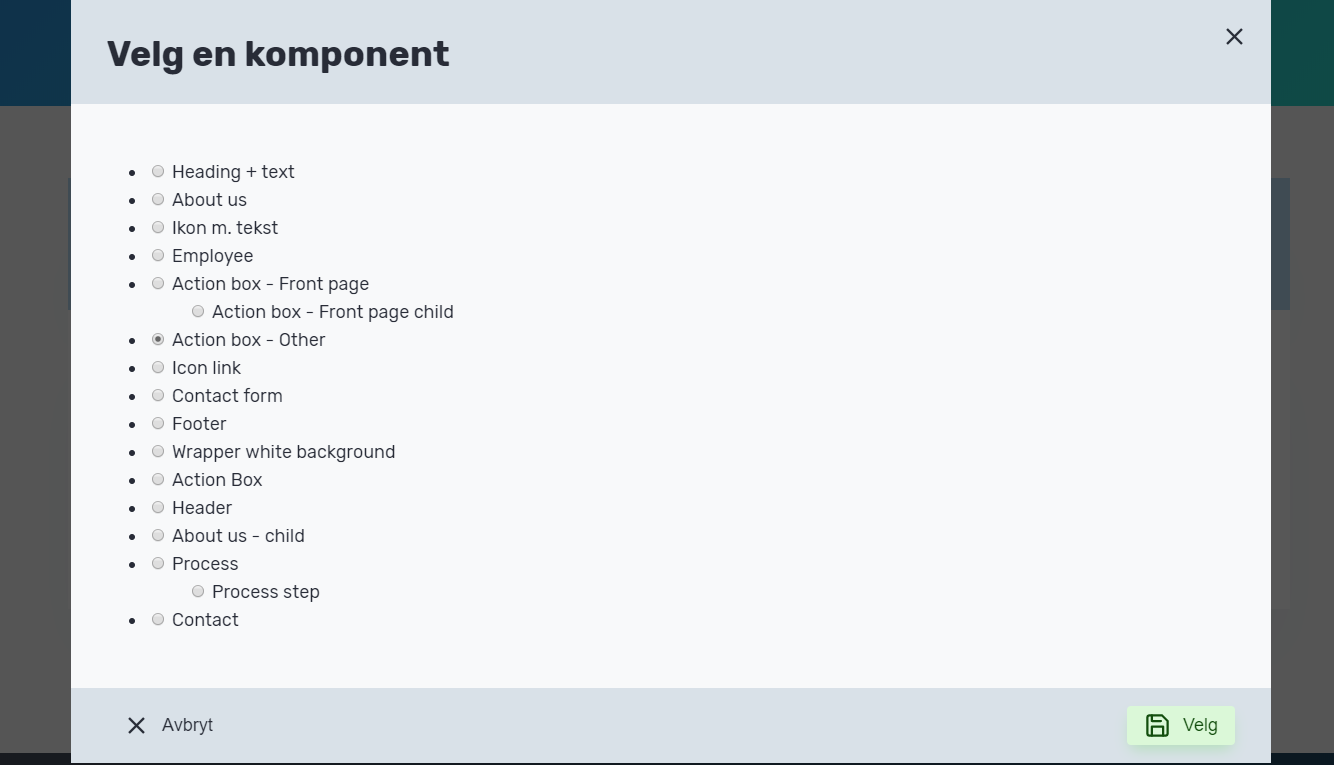
\includegraphics[width=\textwidth]{brukerveiledning/chose-component.png}}
    \label{fig:cms-chose-component}
\end{figure}

Deretter kan feltene fylles med innhold.

\begin{figure}[H]
    \centering
    \frame{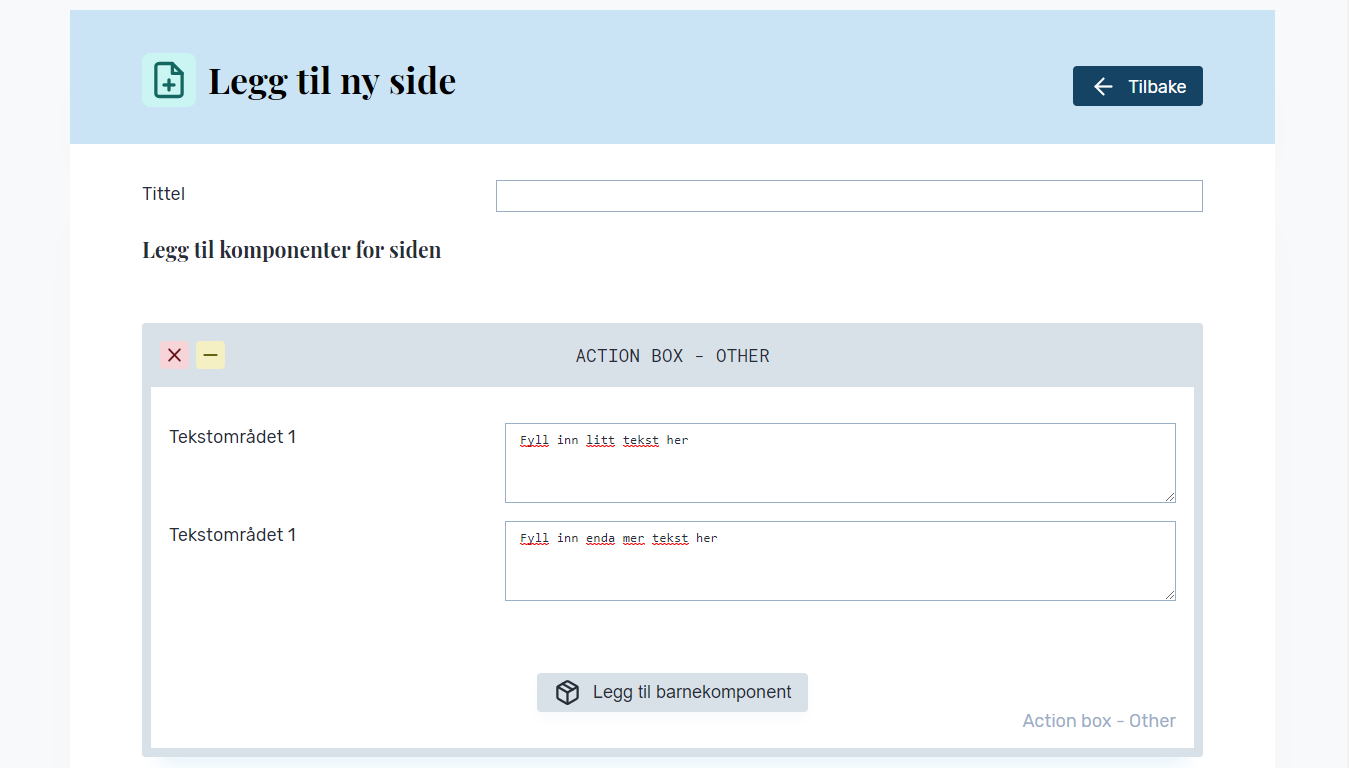
\includegraphics[width=\textwidth]{brukerveiledning/fill-information.png}}
    \label{fig:cms-fill-information}
\end{figure}

For å lagre den nye siden, trykk på \q{Opprett}.

\begin{figure}[H]
    \centering
    \frame{
\includegraphics{brukerveiledning/add.png}}
    \label{fig:cms-add}
\end{figure}

\section{Forelder- og barnekomponenter}
En komponent kan ha flere barn. Dette gjør at de vil havne i samme seksjon på nettsiden. For å legge til et dette, må du trykke \q{Legg til barnekomponent} i den komponenten du ønsker som forelder.

\begin{figure}[H]
    \centering
    \frame{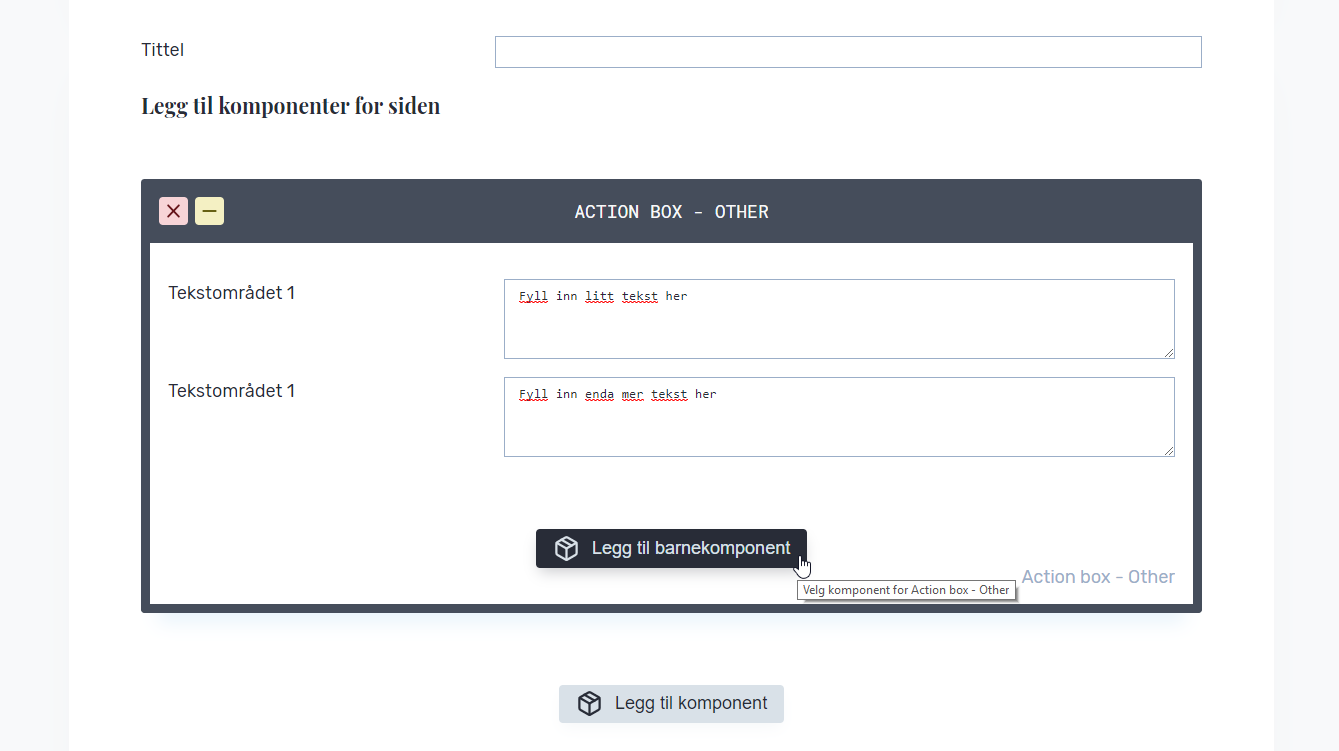
\includegraphics[width=\textwidth]{brukerveiledning/child.png}}
    \label{fig:cms-child}
\end{figure}

\section{Slette en komponent fra en side}
For å slette en komponent eller et barnekomponent fra en side, trykk på det røde krysset til venstre. 

\begin{figure}[H]
    \centering
    \frame{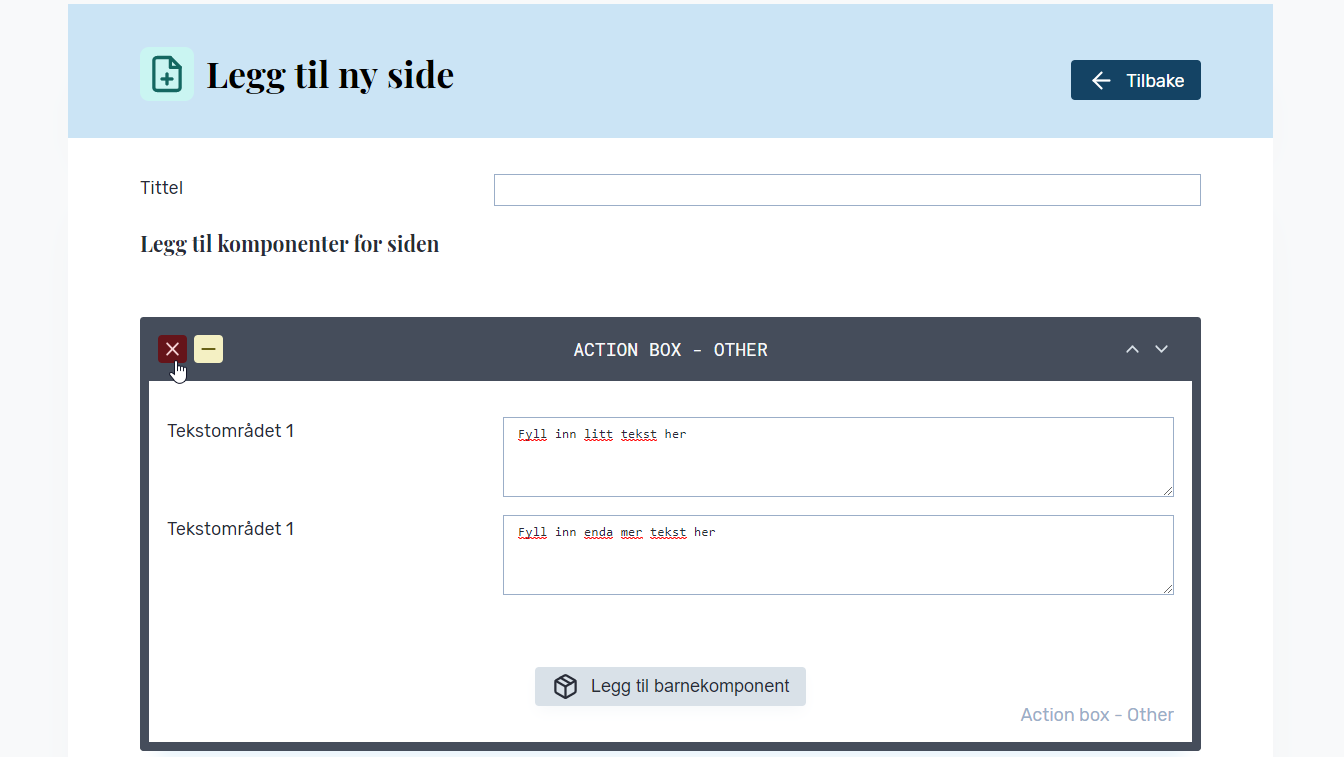
\includegraphics[width=\textwidth]{brukerveiledning/delete-component.png}}
    \label{fig:cms-delete-component}
\end{figure}

\section{Annen nyttig funksjonalitet for komponenter}

Trykk på det gule minus-ikonet (-) for å minimere en komponent.

\begin{figure}[H]
    \centering
    \frame{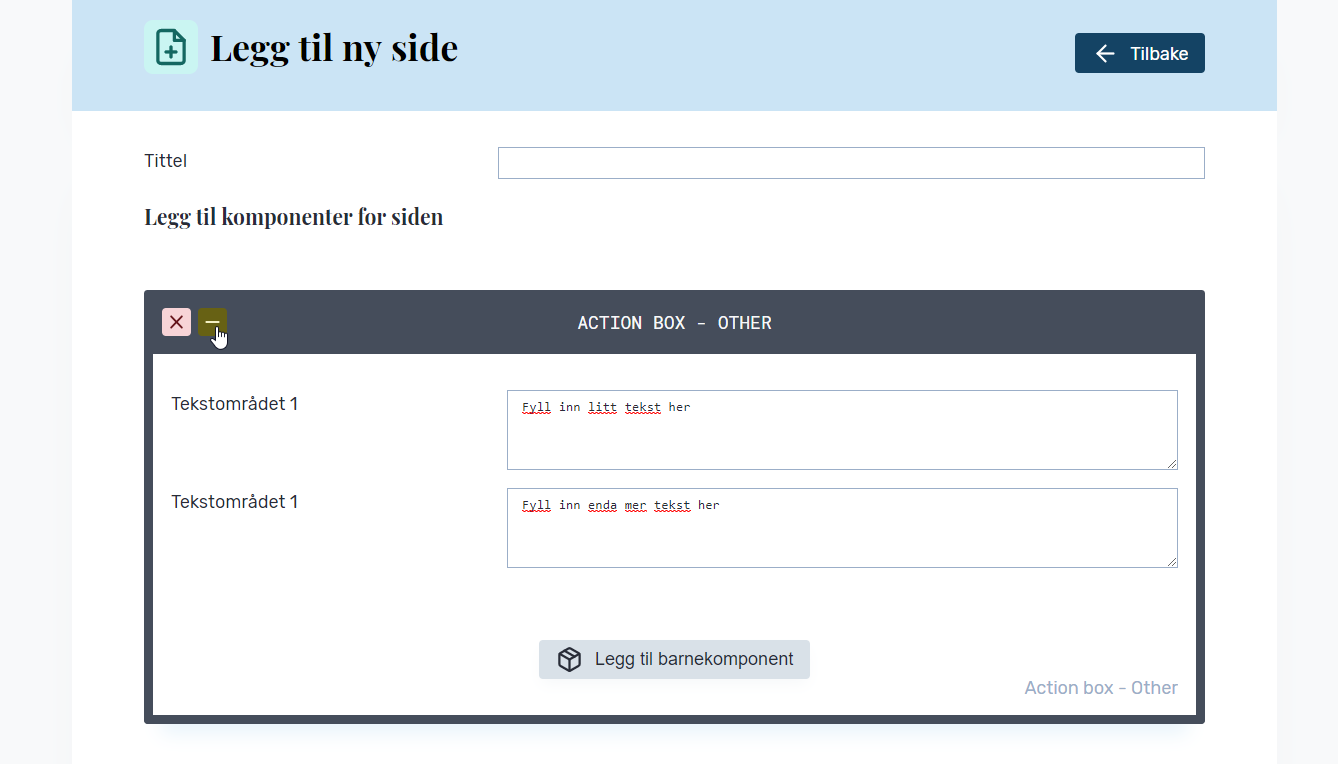
\includegraphics[width=\textwidth]{brukerveiledning/minimize.png}}
    \label{fig:cms-minimize}
\end{figure}

Trykk på det grønne ikonet for å åpne en minimert komponent.

\begin{figure}[H]
    \centering
    \frame{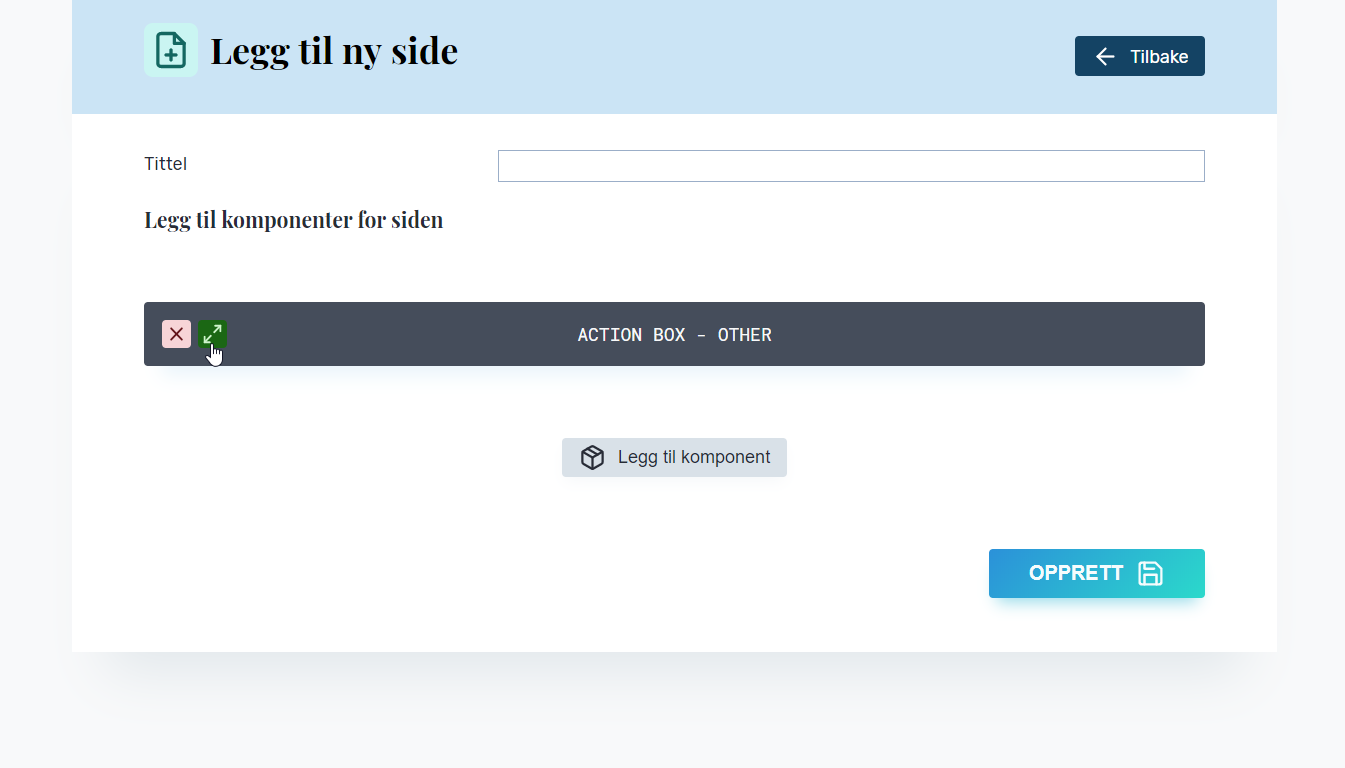
\includegraphics[width=\textwidth]{brukerveiledning/open.png}}
    \label{fig:cms-open}
\end{figure}

Komponentene kommer i den rekkefølgen som blir vist i brukergrensesnittet. Om du ønsker å endre rekkefølgen kan du benytte pilene til høyre. 
\begin{figure}[H]
    \centering
    \frame{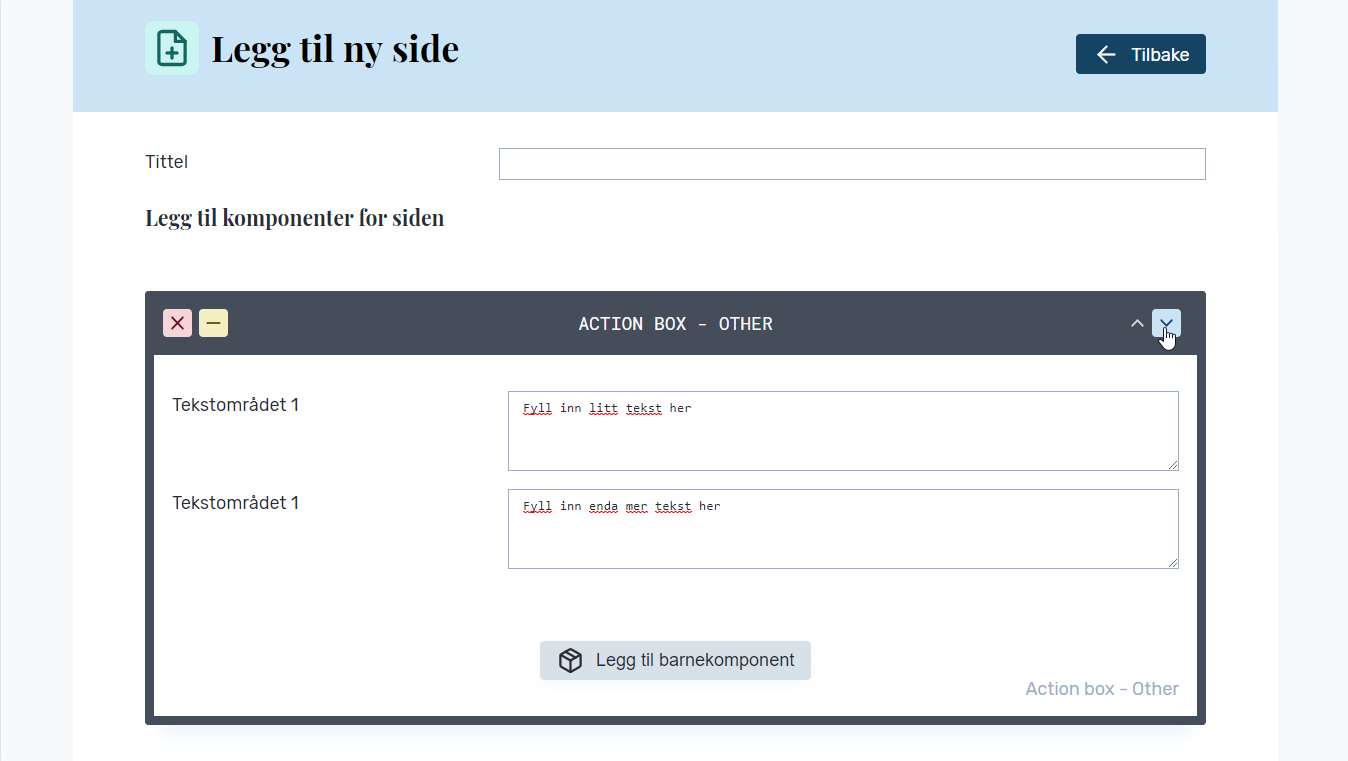
\includegraphics[width=\textwidth]{brukerveiledning/up-down.png}}
    \label{fig:cms-up-down}
\end{figure}

\section{Oversikt over komponenter}
Her kommer en oversikt over de forskjellige komponentene det er mulig å velge mellom:

\subsection{Header}
Headeren er det første som vises på siden. Den bør minst inneholde en tittel. Utover tittelen kan headeren også inneholde et avsnitt med tekst, en knapp samt et tekstfelt under knappen. Figuren under viser headeren til forsiden. Legg merke til at headeren alltd vil ha denne fargen som bakgrunn.

\begin{figure}[H]
    \centering
    \frame{
\includegraphics[width=\textwidth]{brukerveiledning/header-front-page.png}}
    \label{fig:cms-header-front-page}
\end{figure}

\subsection{Action box}
Den hvite boksen med innhold har vi kalt action box. Her kan du velge mellom \q{Action box - forside} som bruker layouten til boksen på forsiden, eller \q{Action box - andre} som har layout som de resterende sidene. For å få til ikonene med tekst, legg til komponenten \q{Ikon m. tekst} som barn av actionboxen.

\begin{figure}[H]
    \centering
    \frame{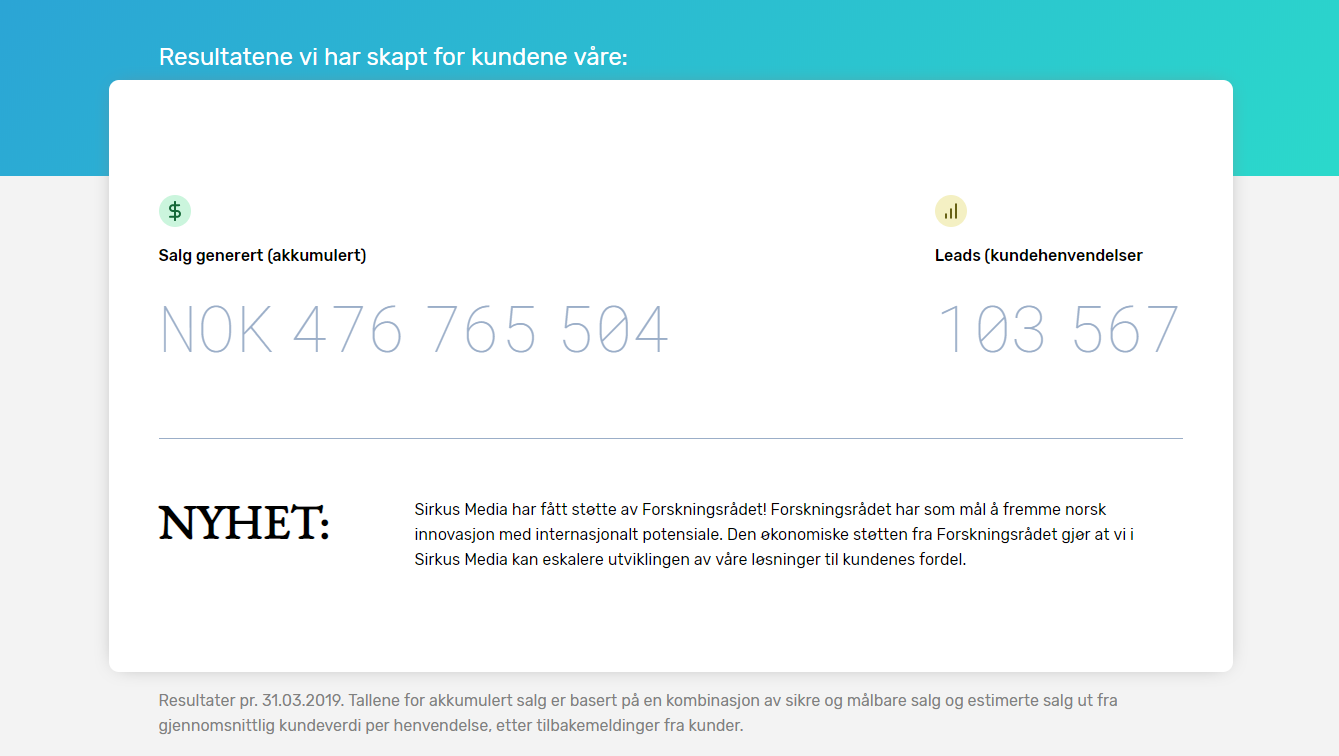
\includegraphics[width=\textwidth]{brukerveiledning/action-box-fp.png}}
    \label{fig:cms-action-box-fp}
    \caption{Action box - forsiden}
\end{figure}

\begin{figure}[H]
    \centering
    \frame{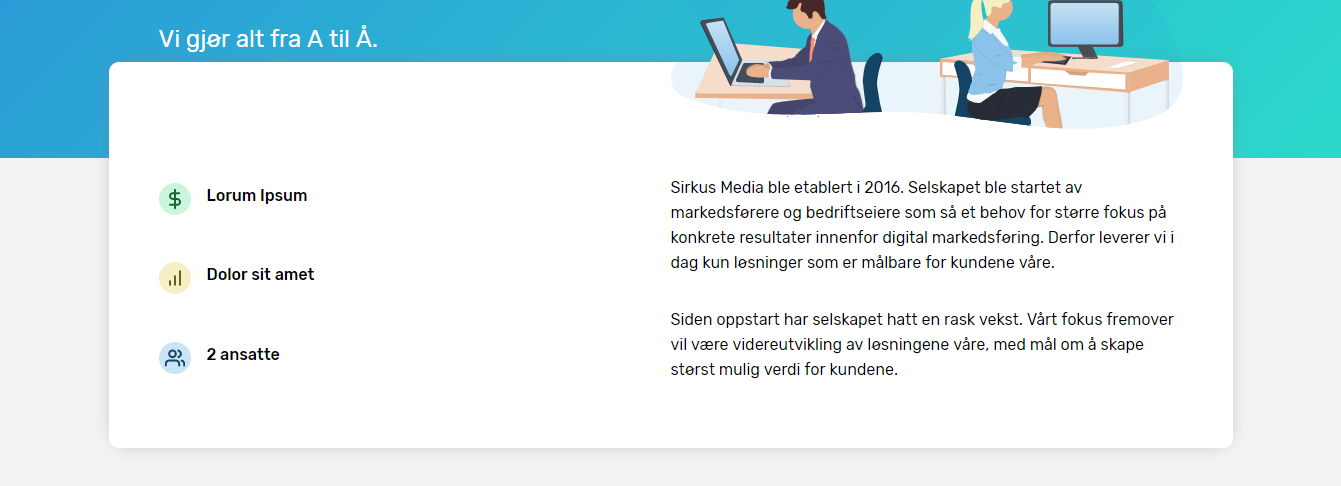
\includegraphics[width=\textwidth]{brukerveiledning/action-box-other.png}}
    \label{fig:cms-action-box-other}
    \caption{Action box - andre. Nb: Bildet tilhører headeren}
\end{figure}

\subsection{Om oss}
\q{Om oss}-komponenten henviser til \q{Om oss}-avsnittet på forsiden. Den kan likevel fint brukes til annen informasjon når du ønsker samme layout med grå bakgrunn.

Det som er spesielt med denne komponenten er at den er helt tom, men fungerer som en slags wrapper for stylingen og gjør at teksten og annet innhold havner der den skal på siden. Derfor må du legge til \q{Om oss - barn} inni denne komponenten for å få samme layout.

\begin{figure}[H]
    \centering
    \frame{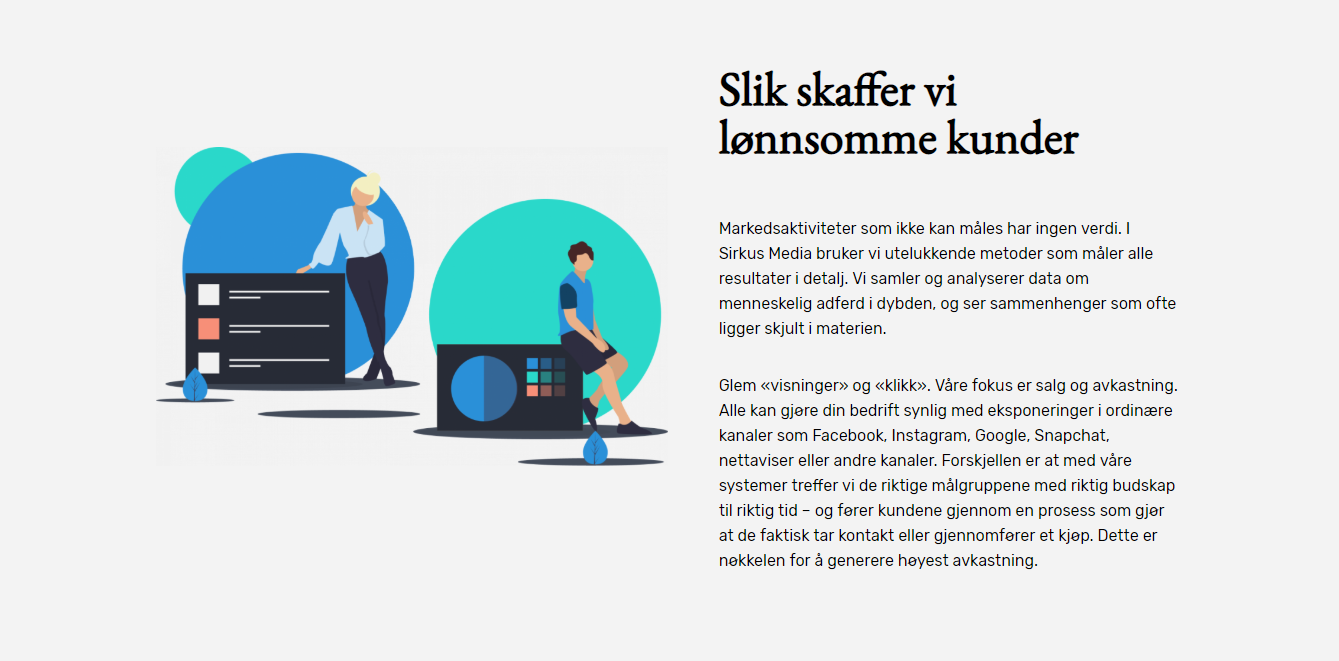
\includegraphics[width=\textwidth]{brukerveiledning/about-us.png}}
    \label{fig:cms-about-us}
\end{figure}

\section{Wrapper - hvit bakgrunn}
\q{Wrapper - hvit bakgrunn} er også en tom komponent som fungerer som en wrapper for stylingen. Forskjellen mellom denne og \q{Om oss} er at denne har hvit bakgrunn. Hvis du for eksempel ønsker en seksjon med overskrift, tekstavsnitt og hvit bakgrunn kan du legge komponenten \q{Overskrift + tekst} som et barn av denne komponenten.

\section{Prosess}
Prosess-komponenten henviser til prosessen. I denne komponenten kan du legge til en hovedoverskrift etterfulgt av så mange steg som er ønskelig. Et steg kan bestå av en overskrift, et tekstområdet og bilde. 

\begin{figure}[H]
    \centering
    \frame{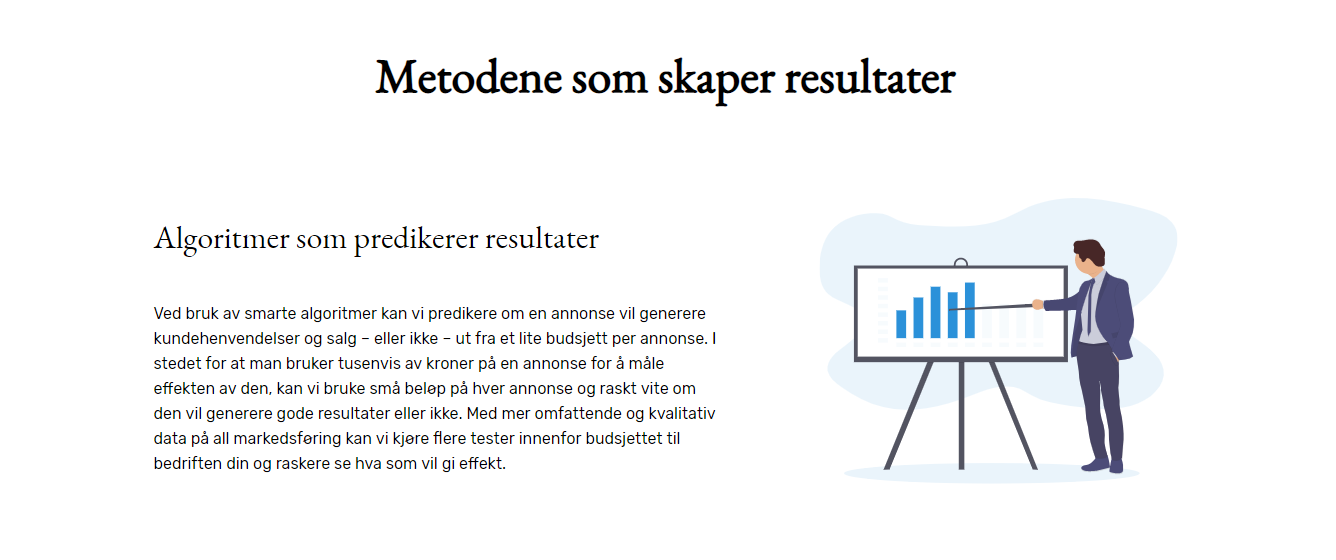
\includegraphics[width=\textwidth]{brukerveiledning/process.png}}
    \label{fig:cms-process}
    \caption{Prosesstittelen + et steg}
\end{figure}

\section{Kontakt}
Kontakt henviser til \q{Kontakt oss}-seksjonen på forsiden med grå bakgrunn. Denne inneholder alltid et kart med lokasjonen til Sirkus Media. Til venstre er det meningen at du skal legge til et barne-komponent, typisk kontaktskjema.

\begin{figure}[H]
    \centering
    \frame{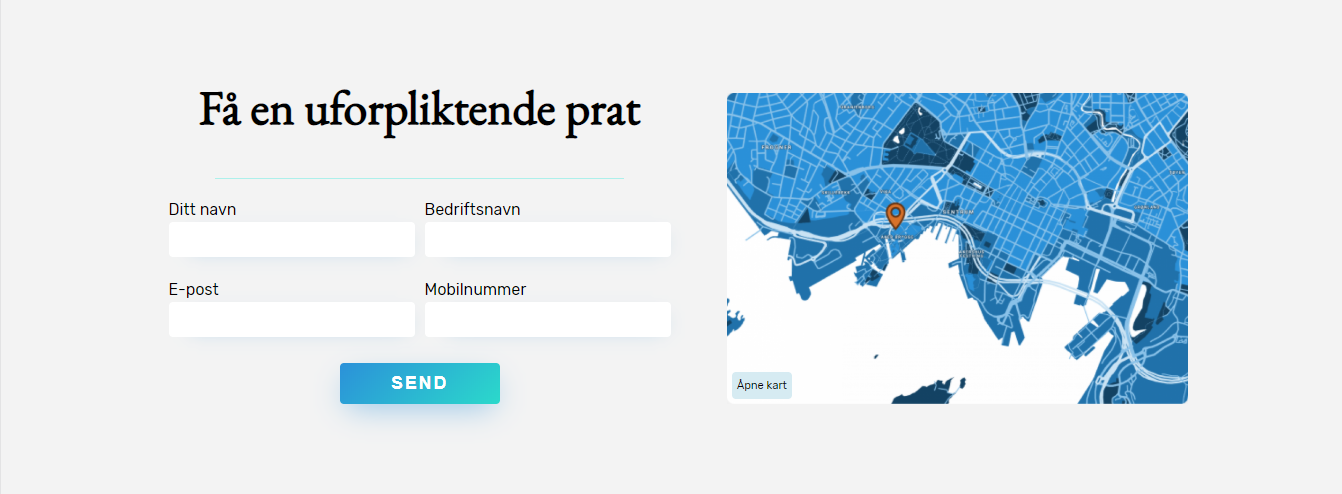
\includegraphics[width=\textwidth]{brukerveiledning/contact.png}}
    \label{fig:cms-contact}
\end{figure}

\section{Kontaktskjema}
Kontaktskjema er selve kontaktskjema.

\begin{figure}[H]
    \centering
    \frame{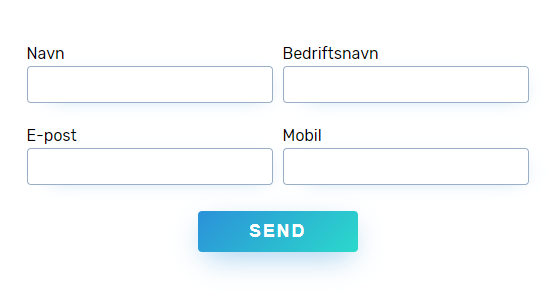
\includegraphics[width=\textwidth]{brukerveiledning/contact-form.png}}
    \label{fig:cms-contact-form}
\end{figure}

\section{Ikon m. tekst}
For å få et ikon ved siden av en tekst bruker du komponenten \q{Ikon m. tekst}. Dette er en komponent som typisk er inni en forelder.

\section{Ikon m. link}
For å få et ikon ved siden av tekst bruker du komponenten \q{Ikon m. link}. Dette er en komponent som typisk er inni en forelder.

\section{Overskrift + tekst}
For å få en overskrift med tilhørende tekst under, bruker du denne komponenten. Dette er også en komponent som ofte vil være inni en forelder. Hvis du ønsker å legge til et tekstområdet kan denne komponenten også brukes til dette, ved å la være å fylle inn overskriften. 

\section{Footer}
Footeren er den seksjonen som befinner seg nederst på siden. 

\begin{figure}[H]
    \centering
    \frame{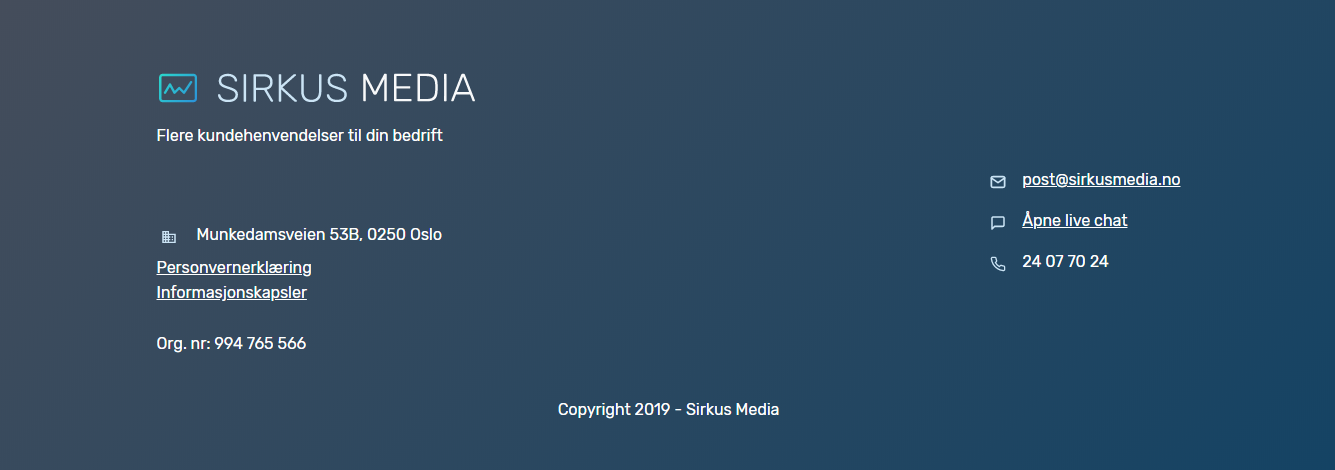
\includegraphics[width=\textwidth]{brukerveiledning/footer.png}}
    \label{fig:cms-footer}
\end{figure}

\section{Tips til hvilke komponenter en side bør inneholde}
For at en side skal ha samme oppsett/layout som de resterende sidene, er det viktig å sette den opp på en bestemt måte. En side bør alltid inneholde disse komponentene, i denne rekkefølgen:
\begin{itemize}
\item Header
\item \q{Wrapper - hvit bakgrunn} eller \q{Om oss}
\item Innholdet, pakket inn i wrapperen som barn. For eksempel \q{Overskrift + tekst}
\item Footer
\end{itemize}

\section{Legge til bilde eller ikon}
For å legge til et bilde eller ikon må du først velge en komponent som innholder felttypen bilde, for eksempel \q{Ikon m. link}. Deretter trykker du på \q{Velg bilde}-knappen.

\begin{figure}[H]
    \centering
    \frame{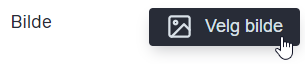
\includegraphics{brukerveiledning/upload-image.png}}
    \label{fig:cms-upload-image}
\end{figure}

 Nå vil det åpne seg et vindu med bildevelgeren. Her kan du velge blant allerede opplastede bilder eller du kan velge å laste opp et nytt fra maskinen din. Dette gjør du ved å trykke på \q{Last opp nytt}-knappen.
 
\begin{figure}[H]
    \centering
    \frame{
\includegraphics{brukerveiledning/upload-new-image.png}}
    \label{fig:cms-upload-new-image}
\end{figure}

\section{Slette bilde eller ikon}
Et bilde kan slettes i bildevelgeren ved å trykke på \q{Slett}.

\begin{figure}[H]
    \centering
    \frame{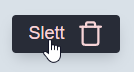
\includegraphics{brukerveiledning/delete-image.png}}
    \label{fig:cms-delete-image}
\end{figure}




\section{Legge til link}
For å legge til en link må du velge en komponent som innholder felttypen link, for eksempel \q{Ikon m. link}. Trykk deretter på \q{Velg link}.
 
\begin{figure}[H]
    \centering
    \frame{
\includegraphics{brukerveiledning/new-link.png}}
    \label{fig:cms-new-link}
\end{figure}

 Nå vil det åpne seg et vindu der du kan velge blant eksisterende lenker eller du kan å opprette en ny. Dette gjør du ved å trykke på \q{Opprett ny}-knappen, som er lokalisert øverst i vindu. 
 
 \begin{figure}[H]
    \centering
    \frame{
\includegraphics{brukerveiledning/add-new-link.png}}
    \label{fig:cms-add-new-link}
\end{figure}

Du må velge om linken er intern eller ekstern. Hvis linken er intern må du skrive inn navn og velge hvilken side den skal gå til. 
 \begin{figure}[H]
    \centering
    \frame{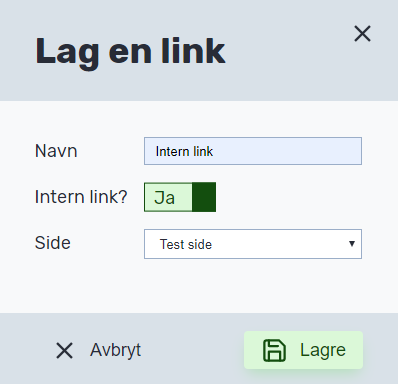
\includegraphics{brukerveiledning/internal-link.png}}
    \label{fig:cms-internal-link}
\end{figure}

Hvis linken er ekstern må du skrive inn navn og legge inn hele URL-en.
 \begin{figure}[H]
    \centering
    \frame{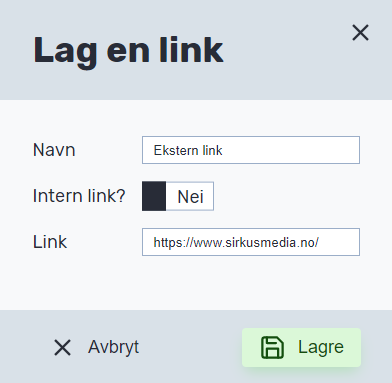
\includegraphics{brukerveiledning/external-link.png}}
    \label{fig:cms-external-link}
\end{figure}

\section{Endre eksisterende side}
For å endre en side, trykk på det grønne \q{Rediger}-ikonet. 

\begin{figure}[H]
    \centering
    \frame{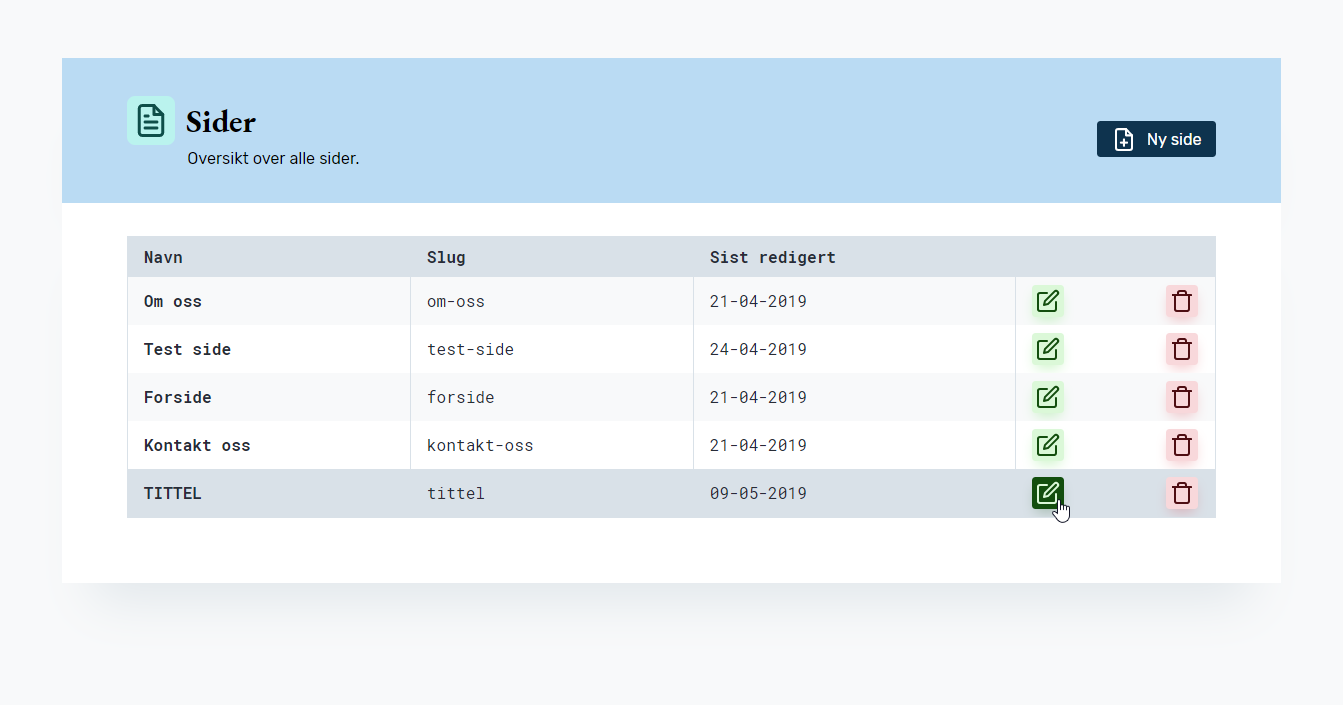
\includegraphics[width=\textwidth]{brukerveiledning/edit.png}}
    \label{fig:cms-edit}
\end{figure}

Deretter kan ønsket innholdet oppdateres. Trykk på \q{Oppdater}-knappen for å lagre.

\begin{figure}[H]
    \centering
    \frame{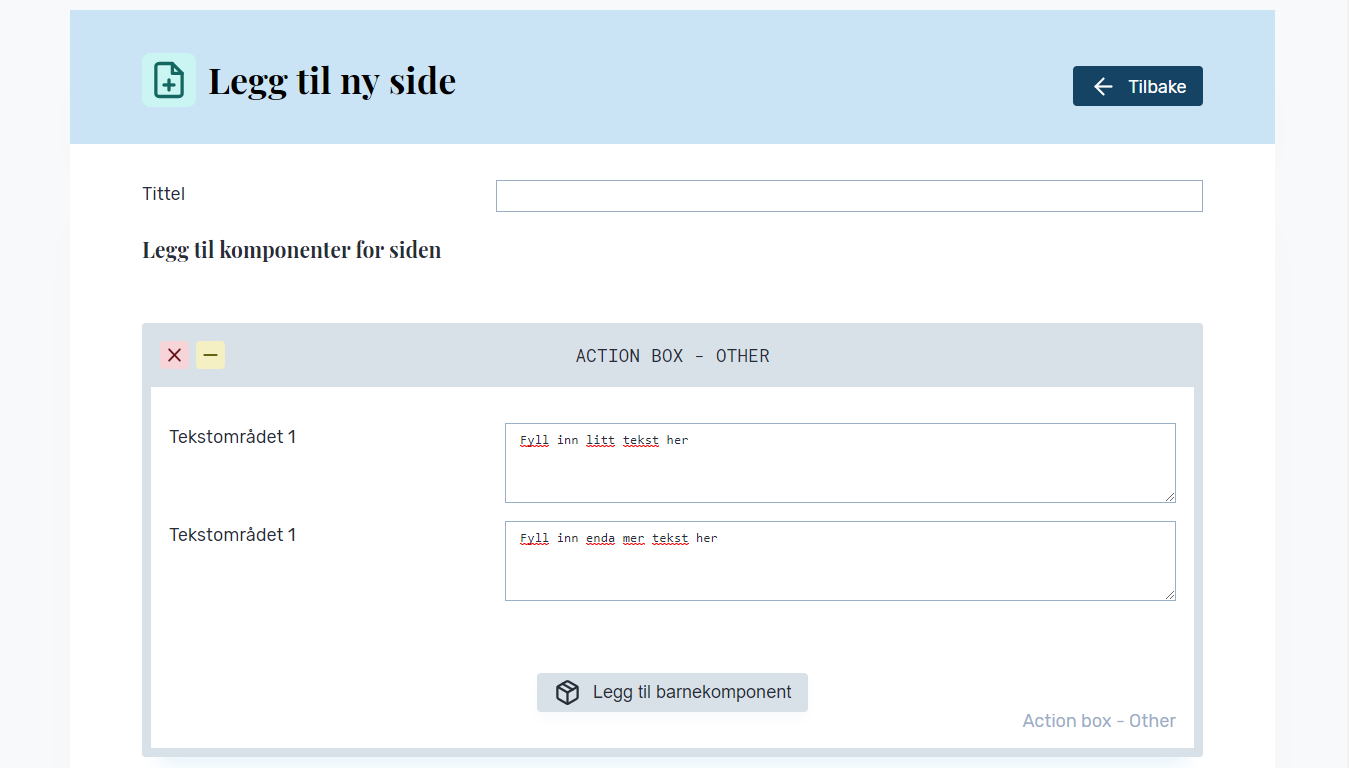
\includegraphics[width=\textwidth]{brukerveiledning/fill-information.png}}
    \label{fig:cms-edit-information}
\end{figure}

\section{Slett eksisterende side}
For å slette en side, trykk på det røde ikonet med søppelbøtte. Deretter vil det dukke opp et bekreftelsevindu. Etter å ha godkjent denne vil siden bli slettet og vil ikke lenger bli vist i oversikten.

\begin{figure}[H]
    \centering
    \frame{
\includegraphics[width=\textwidth]{brukerveiledning/delete-page.png}}
    \label{fig:cms-delete-page}
\end{figure}


\section{Legg til link i meny}
For å legge til en link i menyen, trykk på menypunktet \q{Menyer}. Velg så menyen du ønsker å endre ved å trykke på det grønne ikonet. Da vil du komme til et nytt vindu. Her kan du velge mellom alle linkene som eksisterer og dra den over til \q{Menyens linker}. Trykk på \q{Oppdater} for å lagre.

\begin{figure}[H]
    \centering
    \frame{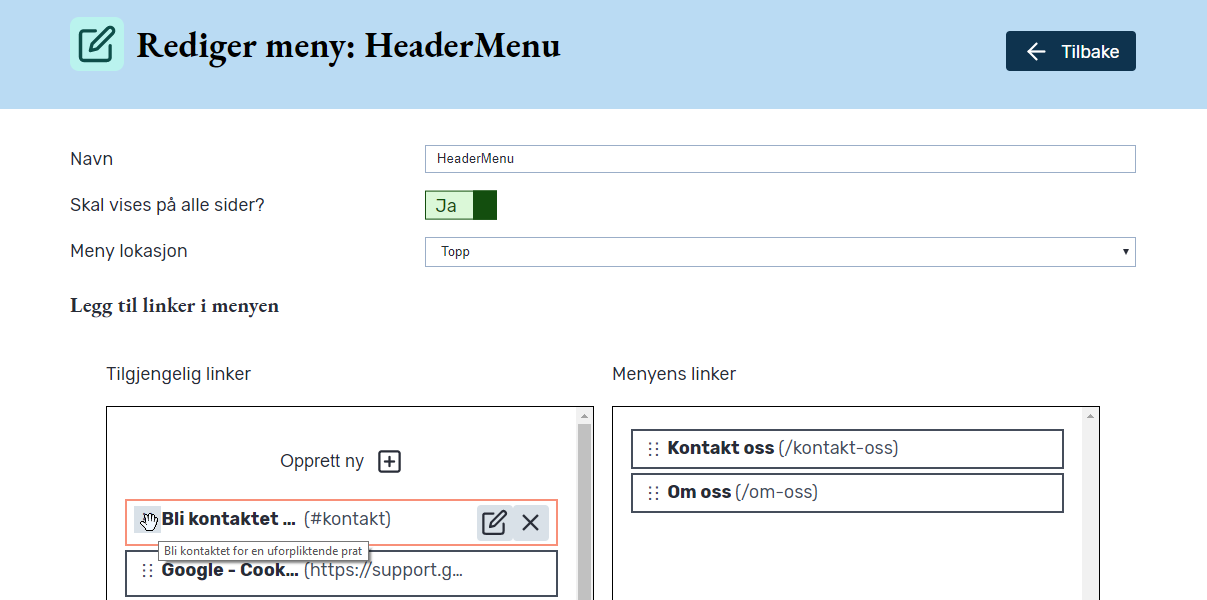
\includegraphics[width=\textwidth]{brukerveiledning/menu.png}}
    \label{fig:cms-menu}
\end{figure}

\section{Endre chat innstillinger}

Trykk på tannhjulet i menyen. Dette tar deg til en oversikt over innstillingene. 

\begin{figure}[H]
    \centering
    \frame{
\includegraphics[width=\textwidth]{brukerveiledning/settings.png}}
    \label{fig:cms-settings}
\end{figure}

Trykk på det grønne rediger-ikonet for chat. I feltet \q{Verdi} kan du lime inn link til scriptet som tilhører chatten. Denne finner du hos din utvalgte chat-leverandør. Deretter kan du trykke \q{Oppdater} for å lagre endringene.

\begin{figure}[H]
    \centering
    \frame{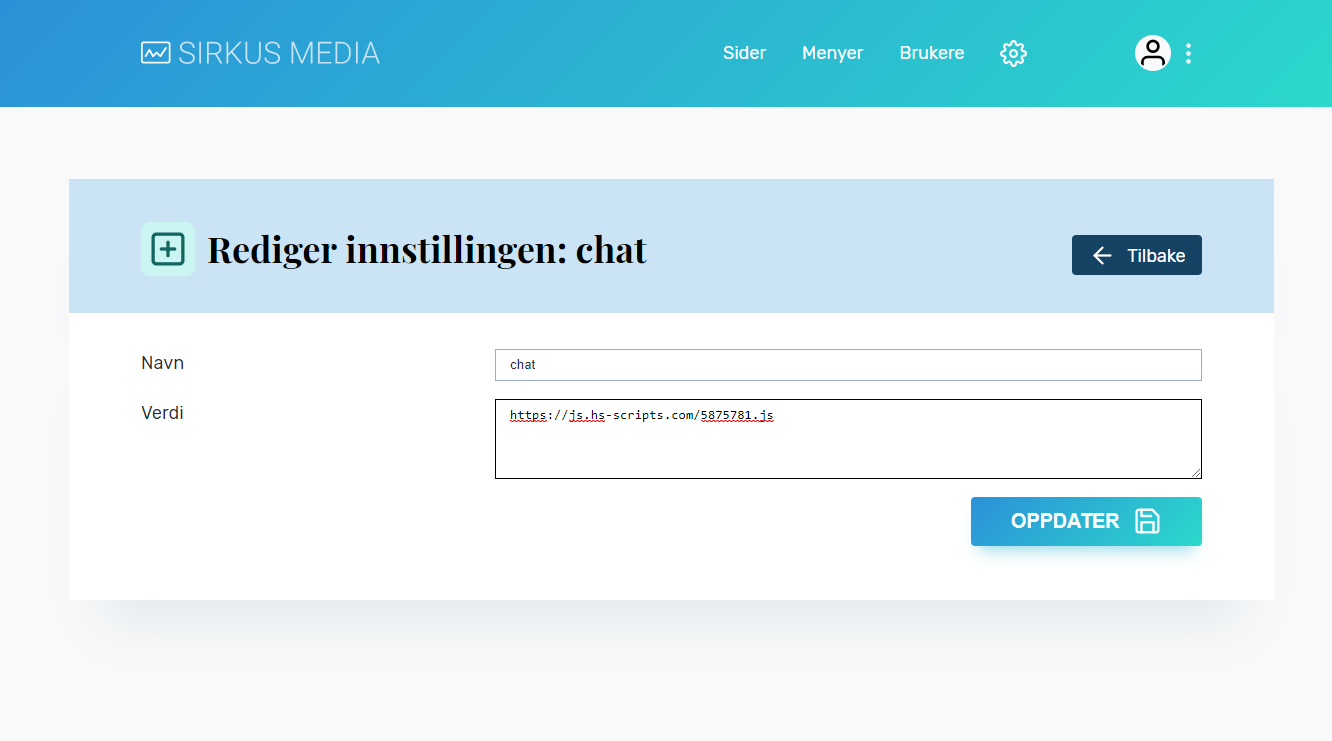
\includegraphics[width=\textwidth]{brukerveiledning/chat.png}}
    \label{fig:cms-chat}
\end{figure}

\section{Endre hvilken e-post kontaktskjema går til}
Første steg er å gå inn på en side som inneholder kontaktskjemaet. Finn så frem til kontaktskjema-komponenten. Her kan du trykke på \q{Velg link}, og legge til linken til utvalgt kontaktskjema-leverandør med riktig e-post. 

\begin{figure}[H]
    \centering
    \frame{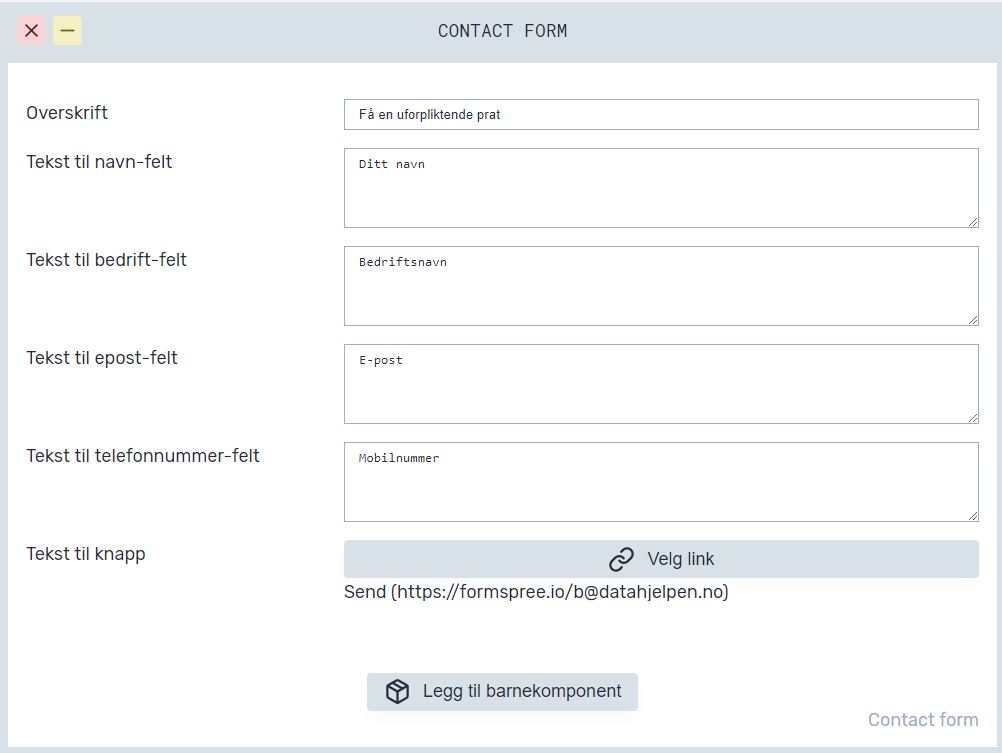
\includegraphics[width=\textwidth]{brukerveiledning/contact-form-email.png}}
    \label{fig:cms-contact-form-email}
\end{figure}


Husk å gjøre endringene på alle sider der kontaktskjema-komponenten blir brukt. Trykk \q{Oppdater} for å lagre endringene. 

\section{Veiledning for superadmin}
Kontrollpanelet til superadmin befinner seg i footeren.

\begin{figure}[H]
    \centering
    \frame{
\includegraphics[width=\textwidth]{brukerveiledning/superadmin.png}}
    \label{fig:cms-superadmin}
\end{figure}

\subsection{Opprette komponent}
Trykk på \q{Komponenter} i superadmin-panelet. Trykk deretter på \q{Ny komponent}

\begin{figure}[H]
    \centering
    \frame{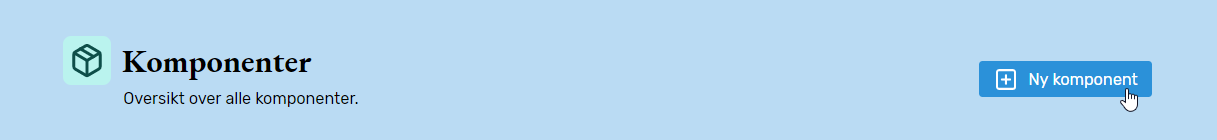
\includegraphics[width=\textwidth]{brukerveiledning/new-component.png}}
    \label{fig:cms-superadmin-add-component}
\end{figure}

Legg deretter til de feltene som er ønsket ved å dra de over til \q{Komponentens felter}. Trykk \q{Oppdater} for å lagre.

\begin{figure}[H]
    \centering
    \frame{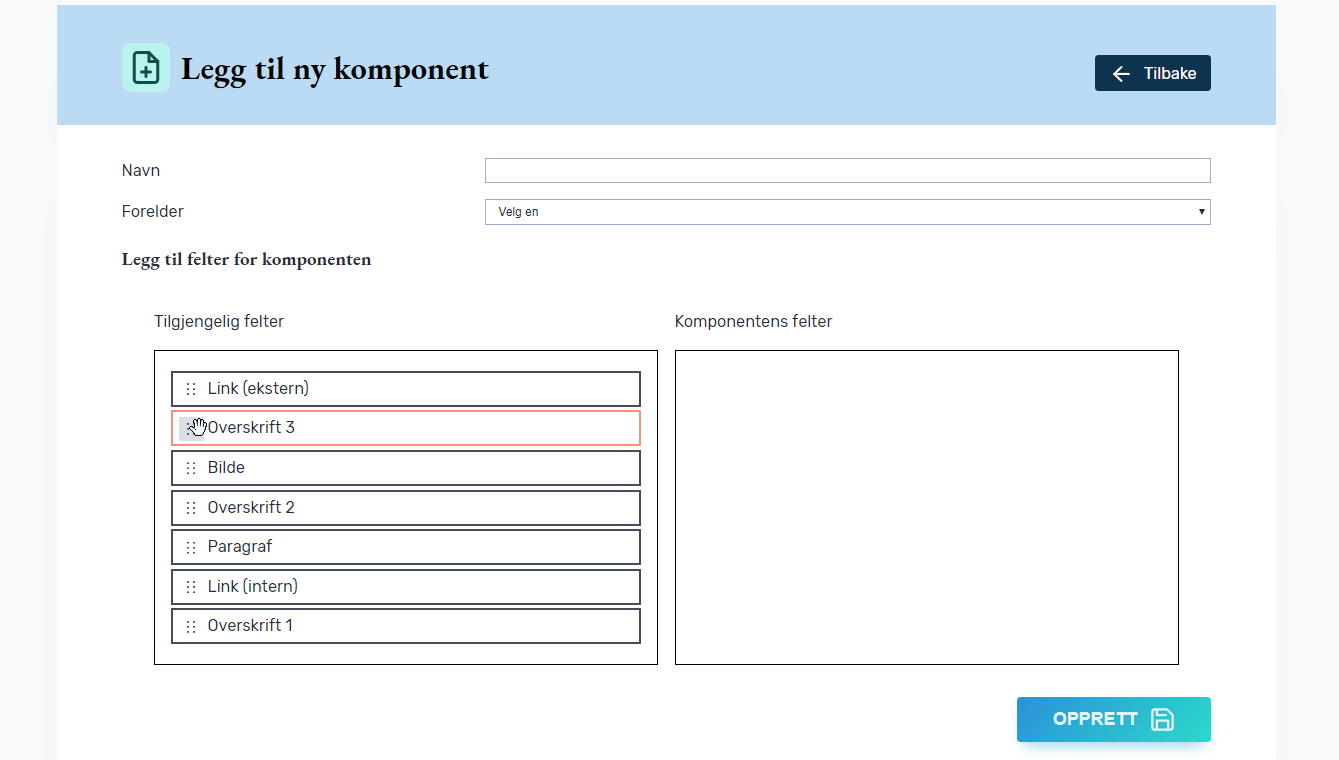
\includegraphics[width=\textwidth]{brukerveiledning/add-field-component.png}}
    \label{fig:cms-superadmin-field-component}
\end{figure}

\subsection{Opprette felt}
Trykk på \q{Felter} i superadmin menyen. Følg samme steg som for å opprette en komponent.

\subsection{Endre felt eller komponent}
Trykk på \q{Felter} eller \q{Komponenter} i superadmin-menyen. Følg samme steg som for å endre en side.